\documentclass{article}

\usepackage{amsmath}
\usepackage{amssymb}
\usepackage{amsfonts}
\usepackage{parskip}
\usepackage{fullpage}
\usepackage{hyperref}
\usepackage{tikz}
\usepackage{pgfplots}
\usepackage{wrapfig}
\usepackage{url}
\usepackage{subfig}
\usepackage{bettelini}
\usepackage[backend=bibtex]{biblatex}

\usetikzlibrary{cd}

\hypersetup{
    colorlinks=true,
    linkcolor=black,
    urlcolor=blue,
    pdftitle={Improved bead sort using Fourier Analysis},
    pdfpagemode=FullScreen,
}

\addbibresource{./references.bib}

\newtheorem{definition}{Definition}[section]
\newtheorem{corollary}{Corollary}[section]
\newtheorem{proof}{Proof}[section]

\title{Improved bead sort using Fourier Analysis}
\author{Paolo Bettelini}
\date{\today}

\begin{document}

\maketitle
\tableofcontents
\pagebreak

\section{Introduction}

\subsection{Abstract}

Bead sort has always been an interesting, but rather useless, sorting algorithm
for natural numbers. It is able to sort numbers without ever directly comparing them.
This paper presents an attempt to make it possibly more efficient
for software when sorting large arrays of numbers.
The resulting algorithm is more efficient (less than \(O(N^2)\)) when sorting a very large array of small integers,
preferably with few distinct elements.

\subsection{Bead sort}

\textit{Bead sort}\cite{beadsort} or \textit{gravity sort}
is a natural sorting algorithm.
This algorithm is primarily used to sort
natural numbers, but can be extended to sort the rationals.

The basic idea is to represent the unsorted natural numbers
in a matrix (\ref{fig:a}), where each columns has \(n\) beads.
We then shift every bead to the right side of the matrix
until they collide with another bead,
as if they were affected by gravity.
The final step is to count the elements in each columns,
forming the final ordered sequence (\ref{fig:b}).

\begin{figure}[h]
    \centering
  
    \subfloat[Unsorted beads]{
        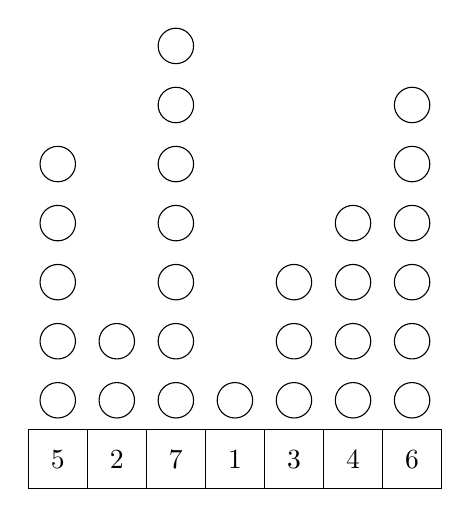
\begin{tikzpicture}[scale=0.75]
            % Draw the array
            \foreach \i/\n in {0/5, 1/2, 2/7, 3/1, 4/3, 5/4, 6/6} {
                \draw (\i,0) rectangle ++(1,1);
                \node at (\i+0.5, 0.5) {\n};
            }
            
            % Beads
            \foreach \i/\n in {0/5, 1/2, 2/7, 3/1, 4/3, 5/4, 6/6} {
                \pgfmathsetmacro{\beads}{\n}
                \foreach \j in {1,...,\beads} {
                \draw (\i+0.5, \j+0.5) circle (0.3cm);
                }
            }
        \end{tikzpicture}
        \label{fig:a}
    }
    \quad\(\longrightarrow\)\quad
    \subfloat[Sorted beads]{
        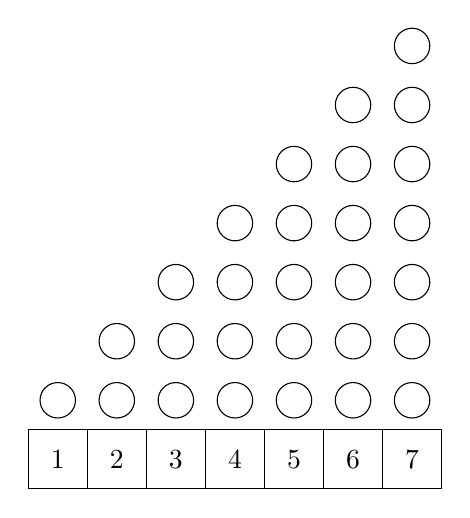
\begin{tikzpicture}[scale=0.75]
            % Draw the array
            \foreach \i/\n in {0/1, 1/2, 2/3, 3/4, 4/5, 5/6, 6/7} {
                \draw (\i,0) rectangle ++(1,1);
                \node at (\i+0.5, 0.5) {\n};
            }
            
            % Beads
            \foreach \i/\n in {0/1, 1/2, 2/3, 3/4, 4/5, 5/6, 6/7} {
                \pgfmathsetmacro{\beads}{\n}
                \foreach \j in {1,...,\beads} {
                \draw (\i+0.5, \j+0.5) circle (0.3cm);
                }
            }
        \end{tikzpicture}
        \label{fig:b}
    }
  
    \caption{Beads matrix for \(S = 5,2,7,1,3,4,6\)}
    \label{fig:both}
\end{figure}

The time complexity of this algorithm, depending on the implementation, ranges from \(O(1)\)
to \(O(P)\) where \(P=\sum S_k\).

\pagebreak

\section{Algorithm}

\subsection{Matrix representation}

\begin{definition}
    Let \(a_n \in {\mathbb{N}}^N\) be the non-empty sequence of \(N\) numbers in \({\mathbb{N}}^*\) to sort,
    indexed as \((a_1, a_2, \cdots, a_N)\).
\end{definition}

\begin{definition}
    A matrix \(M\) with element \(m_{i,j}\) is said to be \textit{numeric} if
    \begin{enumerate}
        \item \(m_{i,j} \in \{0,1\}\).
        \item \(m_{i,j} = 0 \implies m_{a,j} = 0, \quad a \leq i \).
        \item \(m_{i,j} = 1 \implies m_{a,j} = 1, \quad a \geq i \).
    \end{enumerate}
\end{definition}

\textit{Remark.} A numeric matrix is a matrix where each of the columns is made of \(0\)s followed by
some amount of \(1\)s. Thus, each column represents a number in \(\mathbb{N}\)
if the \(1\)s are counted.
A numeric matrix is a representation of the matrix used in gravity sort.

\begin{definition}
    Let \(\tilde{M}\) be the set of all matrices that are numeric.
\end{definition}

\begin{definition}
    Let \(f\colon {\mathbb{N}}^N \to \tilde{M}\) be a non-injective, surjective function
    such that \(f(a_n)\) is defined as the matrix of size \(\max\{a_n\} \times N\)
    with elements \(m_{i,j}\) where
    \[
        m_{i,j} =
        \begin{cases}
            0 & \max\{a_n\} - i > a_j \\
            1 & \max\{a_n\} - i \leq a_j
        \end{cases}
    \]
    which is obviously numeric.
\end{definition}

\textit{Remark.} The function \(f\) transform a sequence of natural numbers into its corresponding
numeric matrix. We are now going to create a function that transforms 
a numeric matrix given by a sequence into a sinusoidal function.
The construction is made such that each row of the matrix represents a frequency
starting at \(\xi=1\) from the bottom up. The amount of \(1\)s in the row
is the magnitude of the frequency.

\textit{Example.} Consider the sequence \(a_n = (5,3,5,6,1,2)\).

\begin{minipage}{0.3\textwidth}
    \begin{flushright}        
    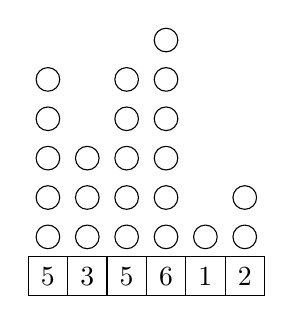
\begin{tikzpicture}[scale=0.5]
        % Draw the array
        \foreach \i/\n in {0/5, 1/3, 2/5, 3/6, 4/1, 5/2} {
            \draw (\i,0) rectangle ++(1,1);
            \node at (\i+0.5, 0.5) {\n};
        }
        
        % Beads
        \foreach \i/\n in {0/5, 1/3, 2/5, 3/6, 4/1, 5/2} {
            \pgfmathsetmacro{\beads}{\n}
            \foreach \j in {1,...,\beads} {
                \draw (\i+0.5, \j+0.5) circle (0.3cm);
            }
        }
    \end{tikzpicture}
    \end{flushright}
\end{minipage}
\hspace{0.5cm}\(\longrightarrow\)\hspace{0.5cm}
\begin{minipage}{0.5\textwidth}
    \[
        6\sin(t) + 5\sin(2t) + 4\sin(3t) + 3\sin(4t)+3\sin(5t)+\sin(6t)
    \]
\end{minipage}

\begin{definition}
    Let \(X(t)\) be a time-dependent function
    \[
        X(t) \triangleq
        \sum_{k=1}^{N}
        \sum_{f=1}^{a_k}
        \sin(ft)
    \]
\end{definition}

\textit{Remark.} The function \(X(t)\) is defined as a naive count of each \(1\) in the numeric matrix.
For each frequency \(\xi\), \(X(t)\) will contain the frequency \(\xi\) with a magnitude equal to
the number of \(1\)s in the row corresponding to \(\xi\).
Many numeric matrices correspond to the same function, since the information of the initial order is lost.

It can be noted that computing \(X(t)\) at some point \(t=k\) has a high time complexity.
A computer needs to add a sine function for each \(1\) in the matrix, meaning
more operations as the amount of numbers increase and as the value of the numbers increase.
Thus, computing \(X(t)\) has a time complexity of \(O(N \cdot P)\) where
\(P=\sum a_n\).

\begin{corollary}
    The function \(X(t)\) is equal to
    \[
        \sum_{k=1}^{N} \frac{\sin(a_k t/2)}{\sin(t/2)} \sin((a_k+1)t/2)
    \]
    for \(t \neq 0\).
\end{corollary}

\begin{proof}
    Note that the naive definition of \(X(t)\) contains a geometric series.
    \begin{align*}
        \sum_{k=1}^{N} \sum_{f=1}^{a_k} \sin(ft) 
        &= \sum_{k=1}^{N} \Im \sum_{f=1}^{a_k} e^{ift} \\
        &= \sum_{k=1}^{N} \Im \left( e^{it} \frac{e^{ita_k}-1}{e^{it}-1} \right) \\
        &= \sum_{k=1}^{N} \Im \left( e^{it} \frac{e^{ia_kt/2}(e^{ia_kt/2} - e^{-ia_kt/2})}
            {e^{it/2}(e^{it/2} - e^{-it/2})} \right) \\
        &= \sum_{k=1}^{N} \Im \left( e^{it} \frac{e^{ia_kt/2}(2i\sin(a_kt/2))}
            {e^{it} (2i\sin(t/2))} \right) \\
        &= \sum_{k=1}^{N} \Im \left( e^{i(a_k+1)t/2} \frac{\sin(a_k t/2)}{\sin(t/2)} \right) \\
        &= \sum_{k=1}^{N} \Im \left(
                ( \cos((a_k+1)t/2) + i\sin((a_k+1)t/2)) \frac{\sin(a_k t/2)}{\sin(t/2)}
            \right) \\
        &= \sum_{k=1}^{N} \frac{\sin(a_k t/2)}{\sin(t/2)} \sin((a_k+1)t/2)
    \end{align*}
\end{proof}

\textit{Remark.} The time complexity of \(X(t)\) can be now reduced to \(O(N)\)
using this representation.

\subsection{Fourier Transform}

\begin{definition}
    Let \(\hat{X}(\xi)\) be the Fourier Transform of \(X(t)\).
    \[
        \hat{X}(\xi)
        \triangleq
        \mathcal{F}\{X(t)\}
    \]
    which is a frequency-dependent function.
\end{definition}

\textit{Remark.} The idea of the algorithm is to apply the Fourier Transform to \(X(t)\)
in order to retrieve the amount of each frequency in the function, thus retrieving
the amount of \(1\)s for each row.
The amount of \(1\)s in the row corresponding to the frequency \(\xi\) is given by \(|\hat{X}(\xi)|\).

\begin{corollary}
    The closed-form for \(\hat{X}(\xi)\) is given by
    \[
        \hat{X}(\xi) =
        \frac{1}{2\pi}
        \sum_{k=1}^{N}
        \,
        \integral[0][2\pi]
        [\frac{\sin(a_k t/2)}{\sin(t/2)} \sin((a_k+1)t/2)e^{-2\pi it\xi}]
        [t]
    \]
\end{corollary}

\begin{proof}
    By the representation of \(X(t)\)
    \begin{align*}
        \hat{X}(\xi) &=
        \frac{1}{2\pi}
        \integral[0][2\pi]
        [e^{-2\pi it\xi}X(t)] [t] \\
        &= \frac{1}{2\pi}
        \integral[0][2\pi]
        [e^{-2\pi it\xi}\sum_{k=1}^{N} \frac{\sin(a_k t/2)}{\sin(t/2)} \sin((a_k+1)t/2)]
        [t]
        \\ 
    \end{align*}
    
    Since \(N\) is finite, we can apply an
    interchange of summation and integration
    \[
        \hat{X}(\xi) =
        \frac{1}{2\pi}
        \sum_{k=1}^{N}
        \,
        \integral[0][2\pi]
        [\frac{\sin(a_k t/2)}{\sin(t/2)} \sin((a_k+1)t/2)e^{-2\pi it\xi}]
        [t]
    \]
\end{proof}

\textit{Remark.} The time complexity of computing this function at a point using its closed-form is \(O(N)\)
and the space complexity \(O(1)\).
Another approach would be to use the Fast Fourier Transform.
The time complexity of the FFT is \(O(N\log(N))\), but we would first
need to allocate a discrete approximation of \(X(t)\) in memory.
The space complexity of this operation would be \(O(\max\{a_n\})\).

\subsection{Sorting Algorithm}

The amount of \(1\)s in each row, computed using the Fourier Transform,
can be used to generate the sorted sequence of numbers.
The principle is the same as the one used during gravity sort:
counting the \(1\)s in each column of the sorted numeric matrix gives the ordered sequence.

For all \(\xi \in {\mathbb{N}}^*\), the frequencies given by
\(|\hat{X}(\xi)|\) are integers, and they follow the property
\(|\hat{X}(\xi)| \geq |\hat{X}(\xi+1)|\).
The first value is always \(|\hat{X}(1)|=N\), since every number in \(a_n\) produces 
the frequency \(1\) of the first row of the numeric matrix (because the sequence is non-empty, every element is at least 1).

In order to retrieve the sorted numbers, we can gradually increase
the frequency \(\xi\) by \(1\) starting at \(\xi=1\). \\
Let \(k=|\hat{X}(\xi)| - |\hat{X}(\xi+1)|\). Whenever \(k \neq 0\)
we consider \(\xi\) to be the next elements in the list of ordered
integers. The element \(\xi\) will be the next in the ordered sequence,
and it will appear \(k\) many times.
Repeat this process until all numbers have been extracted
(\(\xi = \text{max}(S)\) or \(|\hat{X}(\xi)|=0\)).

\textit{Example.} Consider the sequence \(a_n = (5,3,5,6,1,2)\).\\
Then, \(X(t)=6\sin(t) + 5\sin(2t) + 4\sin(3t) + 3\sin(4t)+3\sin(5t)+\sin(6t)\) and

\begin{figure}[ht]
\begin{minipage}{0.5\textwidth}
    \[
        f(a_n) = \begin{bmatrix}
            0 & 0 & 0 & 1 & 0 & 0 \\
            1 & 0 & 1 & 1 & 0 & 0 \\
            1 & 0 & 1 & 1 & 0 & 0 \\
            1 & 1 & 1 & 1 & 0 & 0 \\
            1 & 1 & 1 & 1 & 0 & 1 \\
            1 & 1 & 1 & 1 & 1 & 1
        \end{bmatrix}
    \]
\end{minipage}
\begin{minipage}{0.5\textwidth}
    \centering
    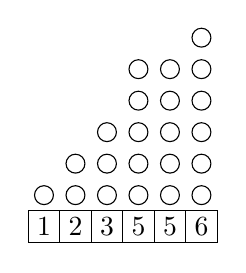
\begin{tikzpicture}[scale=0.40]
        % Draw the array
        \foreach \i/\n in {0/1, 1/2, 2/3, 3/5, 4/5, 5/6} {
            \draw (\i,0) rectangle ++(1,1);
            \node at (\i+0.5, 0.5) {\n};
        }
        
        % Beads
        \foreach \i/\n in {0/1, 1/2, 2/3, 3/5, 4/5, 5/6} {
            \pgfmathsetmacro{\beads}{\n}
            \foreach \j in {1,...,\beads} {
            \draw (\i+0.5, \j+0.5) circle (0.3cm);
            }
        }
    \end{tikzpicture}
    \caption{Sorted numerical matrix of \(a_n\)}
\end{minipage}
\end{figure}

The values of \(|\hat{\xi}|\) are easy to guess by looking at \(X(t)\).

\begin{center}
\begin{tikzcd}
    \hat{X}(1)=6 \arrow[r, "k=1"', bend right] & \hat{X}(2)=5 \arrow[r, "k=1"', bend right] & \hat{X}(3)=4 \arrow[r, "k=1"', bend right] & \hat{X}(4)=3 \\
    \hat{X}(5)=3 \arrow[r, "k=2"', bend right] & \hat{X}(6)=1 \arrow[r, "k=1", bend right]  & \hat{X}(7)=0 \arrow[r, "k=0"', bend right] & \hat{X}(8)=0
\end{tikzcd}
\end{center}

Note that \(\hat{X}(\xi) = 0\) for \(\xi > 6\).
We are looking for the cases where \(k \neq 0\). \\
\begin{enumerate}
    \item At frequency \(1\), the value \(6\) decreases to \(5\), meaning that the first sorted element is \(1\).
    \item At frequency \(2\), the value \(5\) decreases to \(4\), meaning that the next sorted element is \(2\).
    \item At frequency \(3\), the value \(4\) decreases to \(3\), meaning that the next sorted element is \(3\).
    \item At frequency \(5\), the value \(3\) decreases to \(1\), meaning that the next sorted elements are the number \(5\)
    repeated two times (\(k=3-1=2\)).
    \item At frequency \(6\), the value \(1\) decreases to \(1\), meaning that the last sorted element is \(6\).
\end{enumerate}

It is important to note that duplicate numbers,
such as \(5\) in this case, collapse under the same
point in \(|\hat{X}(\xi)|\).

\section{Space and time complexities}

The ordered elements need to be retrieved from \(\max\{a_n\}\) values of
\(|\hat{X}(\xi)|\). Let \(A\) be the average distance between two consecutive sorted
elements in \(a_n\) and \(D\) be the amount of distinct elements in \(a_n\).\\
Note that \(D \cdot A \approx \max\{a_n\}\) for an homogeneous distribution.

When using a closed-form for \(\hat{X}\), the retrieval has time complexity
\(O(N \cdot \max\{a_n\})\) if we scan the frequencies linearly.
It is possible to optimize this operation using a binary search or similar approaches.
The binary search will be used to reach the next point where \(|\hat{X}|\) decreases.
The binary search will be repeated \(D\) times, and for each time
it will travel approximately \(A\) values. Since computing each value has cost \(O(N)\),
and the cost of a binary search is \(O(\log(N))\),
the final time complexity is \(O(D \cdot N \log(A))\).
The space complexity is always \(O(1)\).

\section{Appendix}

The time complexity of \(O(D \cdot N \log(A))\), where \(A\)
is the average distance between two consecutive sorted
elements and \(D\) is the amount of distinct elements in the array,
can be sometimes advantageous.

An important property of this algorithm is its case-independence.
The initial orderliness of the array (best case, average case and best case)
do not affect the performance.

\pagebreak

\begin{figure}[ht]
\centering
\begin{tikzpicture}
    \begin{axis}[
        xmode=log,
        ymode=log,
        xlabel={array size [\textit{bytes}]},
        ylabel={time [\textit{ms}]},
        ]
        \addplot table [x=a, y=b, col sep=comma] {data.csv};
        \addplot table [x=a, y=c, col sep=comma] {data.csv};
    \end{axis}
\end{tikzpicture}
\caption{Time complexity: gravity (blue) vs tim sort (red)}
\end{figure}

\nocite{*} % cite all entries

\printbibliography
\listoffigures

\end{document}
